\chapter{Deta analysis}
\label{chapter:analysis}
The HADES experiment has performed a proton-proton experiment with beam kinetic energy 3.5 GeV in September 2018. Data collected during this experperiment allowed to conduct a series of analysis devoted to hypererons [ref]. In this thesis the next step in hyperon studies is presented. The four particles $\p \pim \pip \pim$ final state was analyzed. Is allows to reconstruct the inclusive signal of $\Ls$ and $\Lz \Kz$ signal. The obtained results were compared with previous, exclusive measurements and used to constrain simulation of a new esperiment devoted to hyperon studies \ref{chapter:simulations}.

All methodes developed for pp@3.5 GeV experiment were used for deta from pNb@3.5GeV experiment. A simirar analysis ..

\section{Paricles identyfication}
The HADES detector allows for two complementary methodes of particles analysis. A first of them bases on particles time of flight measured in the TOF detectors and particle's momentum measured in the MDC. A second methode bases on MDC exclusively and uses combide information about particles' momentum and energy losses. The first one is favoured due to better precision, however a limited geometrical of the TOF detectors reduces detection efficirncy by a factor 0.8 for each particle. In case of four particles final state, discussed in this thesis, a total loss caused by the TOF detectors  can reach 60\% of all detected particles. For that reason the $\frac{de}{dx}$ vs. momentum identyfication metode was used. Cuts were opimized in Munich group involved in HADES experiment and described in.[ref].
\section{Absolute normalization}
\label{sec:normalization}
An integrated luminosity for the pp experiment was calculated by a pp elastic scattering. It was
\begin{equation}
  L^{int}=3.13 \cdot 10^8 mb^{-1}.
\end{equation}
Thanks to a full scale simulation performed in HYDRA framework it is posible to get a total detection efiiciency for given reaction. Together with a luminocity its provide an ecpected count rate for each channel
\begin{equation}
  N^{\mathrm{expected}}_{pp\rightarrow X}=\frac{N_{\mathrm{detected}}}{N_{\mathrm{Simulated \; in \;} 4 \pi} \cdot 3} \cdot \sigma_{pp\rightarrow X} \cdot L.
\end{equation}
The factor 3 in denominator is connected with a trigger down-scaling. For a hadronic channels each 3th triggered event was seved on tapes. A list of the \css used in following analysis are in \ref{tab:channels}. 
\begin{table}
    \centering
  \caption{List of the channels considered in following chapter. Numbers from 3 up to 10 indicates reactions containing $\p \pim \pip \pim$ in a final state. They are treated as a possible background channels. All values taken from \cite{hades_inclL_35}.}
  \label{tab:channels}
  \begin{tabular}{rll}
    \hline
    no. &Channel & $\sigma$ [$\mu \barn$]\\
    \hline
    \hline
    \multicolumn{3}{c}{3-body reactions} \\
    \hline
    1 & $\Lz \p \Kp$&$35.26 \pm 0.43 ^{+3.55}_{-2.83}$\\
    2 & $\Sz \p \Kp$&$16.5 \pm 20\%$\\
    3 & $\Lz \Dpp \Kz$&$29.45\pm 0.08 ^{+1.67}_{-1.46}\pm 2.06$\\
    4 & $\Sz \Dpp \Kz$&$9.26 \pm 0.05 ^{+1.41} _{0.31}\pm 0.65$\\
    5 & $\Sigma(1385)^+ \p \Kz$&$14.05 \pm 0.05 ^{+1.79}_{-2.14}\pm 1.00$\\
    6 & $\Dpp \Lss \Kz$&$5.0\pm 20\%$\\
    7 &$\Dpp \Ss \Kz$& $3.5 \pm 20\%$\\
    8 &$\Dp \Sigma(1358)^+ \Kz$&$2.3 \pm 20\%$\\
    \hline
    \multicolumn{3}{c}{4-body reactions} \\
    \hline
    9 &$\Lambda \p \pip \Kz $& $2.57 \pm 0.02 ^{+0.21}_{-1.98}\pm 0.18$\\
    10&$\Sz \p \pip \Kz$& $1.35 \pm 0.02 ^{+0.10}_{-1.35}\pm 0.09$\\
    \hline
  \end{tabular}
  
\end{table}

\section{Event selection}
Among all registered events only these with at least four charged particles (two positive and two negative) has been registered in the HADES. In case of situation when detector registered more particles the combination with the lowest $\chi^2$ was taken. ...
\section{Reaction kinematics}
\label{section:kinematics}
A next step after an event selection  was a look into a missing mass spectrum of all analized events. The analized reaction consist of four particles $\p \pim \pip \pim$. In case of signal channel it is produced via reaction
\begin{equation}
  \p\p \rightarrow \p \Kp \Ls.
\end{equation}
The smallest missing mass for the signal channel is $\Sqs - \Ls_{mass}= 1432$ MeV, It seperate the signal channel from most of the background channels well.  The missing mass spectrum is presented in fi.g \ref{fig:missMass}. A resonanse behavour around 1200 MeV is cleary visible. From the charge conservation rule missing particles have to have a total charge +2. 

\begin{figure}[hb]
  \centering
  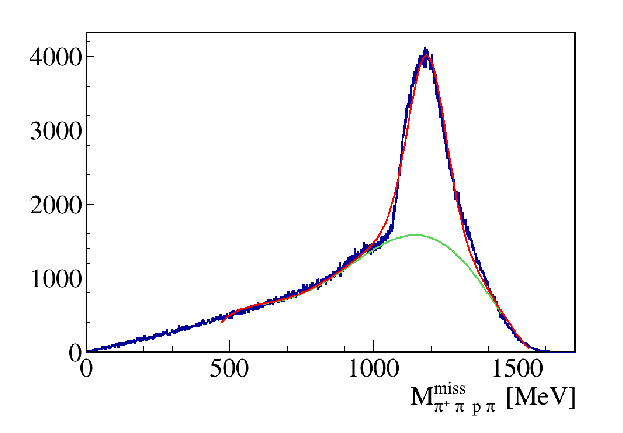
\includegraphics[width=0.9 \linewidth]{Chapter_analysis/missMass.eps}
  \caption{The missing mass of $\p \pim \pip \pim$ system. The resonance behavour around 1200 MeV is cleary visible. The read line represents sum of signal (a Voigt function) and a background (5-th order polynomial) fit. Fited Voigt function gives following parameters: $\bar{M}=1186$ MeV, $\sigma=61$ MeV, $\Gamma=$20 MeV.}
  \label{fig:missMass}
\end{figure}


Becouse in HADES energy regime almost all pions are produced via resonances it was expected that together with $\Dpp$ visible in missing mas a simiral signal should be visible in $\p \pip$ invariant mass spectrum. Indeed, as it is shownn in fig. \ref{fig:dpp2D} most of the background comes from coreleted source. The figure shows also that a cut on missing mass > 1432 MeV remuves a significant part of a background events.

\begin{figure}[hb]
  \centering
  %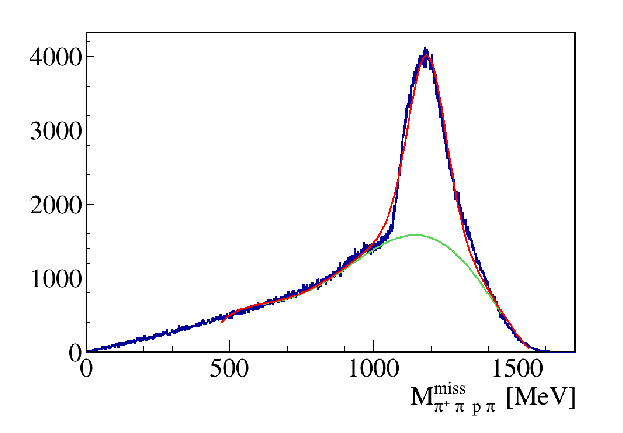
\includegraphics[width=0.9 \linewidth]{Chapter_analysis/missMass.eps}
  \caption{The missing mass of $\p \pim \pip \pim$ system vs. invariant mass of a $\p\pim$ system. It is creary visible that most of the bacground comes from corelated source of two $\Dpp$ production. Such situation helps to easy discriminate most of the background.}
  \label{fig:dpp2D}
\end{figure}

\section{The $\Lz$ Reconstruction}
The next step of the analysis after a missing mass cut was a $\Lz$ reconstructiion. In previous HADES experiments the reconstruction bases on a set of geometrical cuts. Their role was to increase signal-to-background ratio utlizing a $Lz$ decay gemetry. Because the $\Lz$ decasys via week interactions its livetime is relatively long :$c\tau = 7.89 cm$ \cite{PDG}. That may be used to discriminate an out of target vertex from a background originates from a target.

As it was shown in \ref{section:kinematics} an avaliable phase-space for $\Ls$ production for a $E_k=3.5$ GeV is very limited. An inlusive analysis performed in \cite{hades_L1520} has measured N events of $Ls$ after all cuts. To impruve statistics, and also axminate new reconstruction methodes in following analysis a neural network was used to replace the geometrical cuts. Details about used methode are explaned in chapter \ref{chapter:NN}.

The opitimalized neural network enhanced a signal to bacgkround ratio from ??? without any topological cuts to ???. A $\Lz$ signal obtained in this way was used for a next steps of analysis: the $\Ls$ analysis (chapter \ref{section:Ls}) and asocieted $\Lz \Kz$ production (chapter \ref{section:LzKz});
\section{The $\Ls$ Reconstruction}
\label{section:Ls}

\subsection{Side-band analysis}
\section{The $\Lz \Kz $reconstruction}
\label{section:LzKz}
Because of the conservation low a $\Lz$ has to be produced with some anti-strange particle. The lightest option is a $\Kz$ meson, which decays in 69.2\% into $pip pim$ pair \cite{PDG}. For that reason a $\Lz \Kz$ signal is expected to be a significant part of the $\Lz \pip \pim$ final state.

After the $\Lz$ reconstruction two spectra were drown: a) a $\pip \pim$ invariant mass spectrum for events $1006<M^{inv}_{\p \pim}<1026$ and b) a $p pim$ invariant mass for $480 MeV<M^{inv}_{\pip \pim}<500 MeV$. The same analysis chain was used to analyzed all channels from \ref{tab:channels} which contains $\Lz$ and $\Kz$. 

Using a procedure described in \ref{sec:normalization} the simulation was compared with experimental data (see \ref{fig:K0L0}). The simulation describes well a yeld of $\Kz$ and $\Lz$ produced in experiment, aldough it does not describe the background shape. ?? 

\begin{figure}[hb]
  \centering
  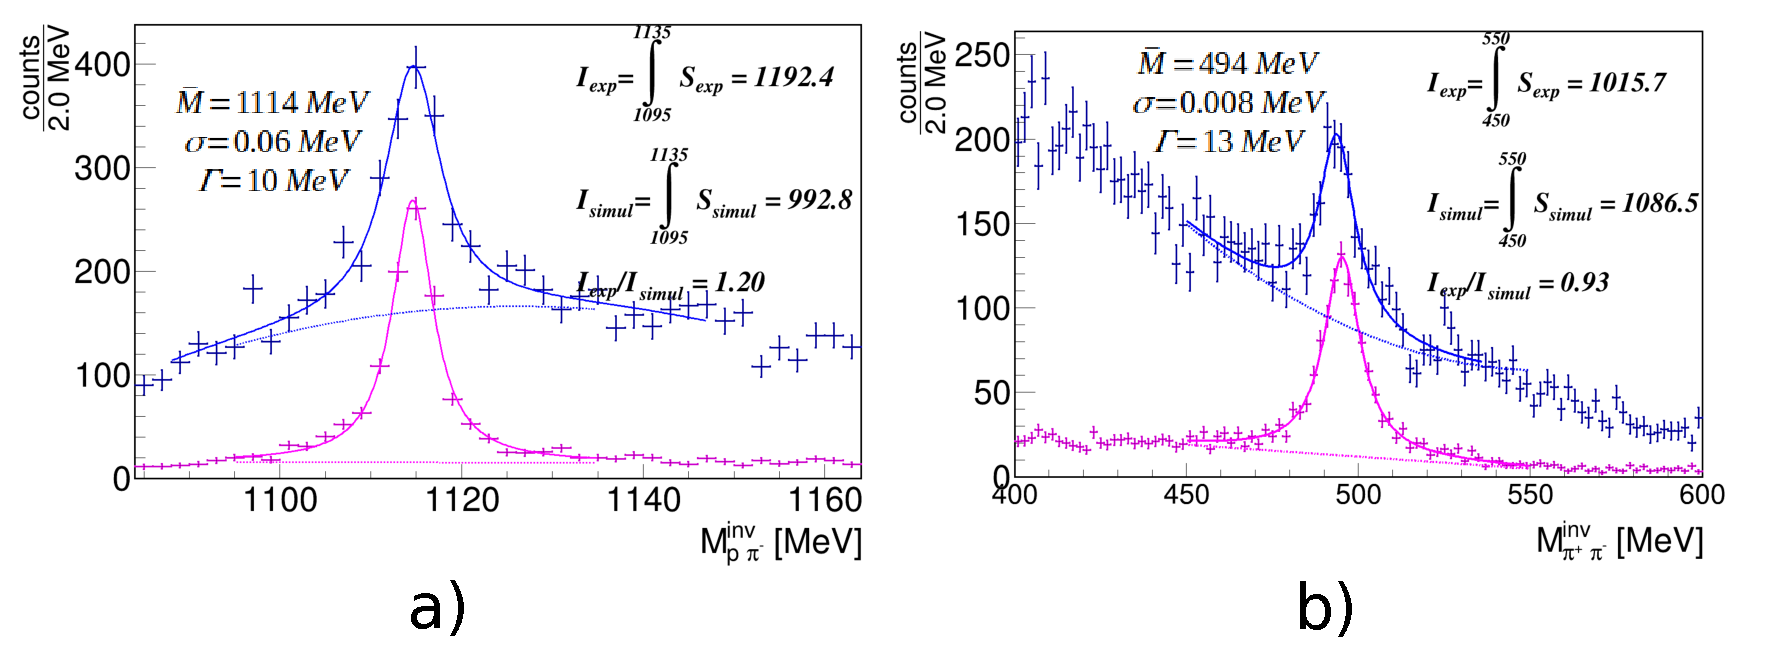
\includegraphics[width=0.9 \linewidth]{Chapter_analysis/K0L0.eps}
  \caption{The results for $\Lz \Kz$ asocieted production. Blue point reprezents experimental data, magenta a sum simulated channels. For both: the simulation and the experimental data a Voigt function was fited. Than a total signal yeld between simulation and experiment was calculated.}
  \label{fig:K0L0}
\end{figure}


\section{results from p Nb experiment}